\newchapter{c:phaseMons}{Phase Monitor Performance}

This is the introductory text.

\newsection{s:monElectronics}{Phase Monitor Electronics}

\newsection{s:monSigResponse}{Signal Response Measurements}

\subsection{Saturation}
\label{ss:monSaturation}

\subsection{Cross-Talk}
\label{ss:crossTalk}

\newsection{s:monCalibrations}{Calibrations}

\subsection{Procedure}
\label{ss:calProcedure}

\subsection{Single Sample Results}
\label{ss:calSingSamp}

\subsection{Multi-Sample Results}
\label{ss:calMultiSamp}

\newsection{s:digNoise}{Digitiser Noise}

\subsection{On FONT5 Board}
\label{ss:font5Noise}

\subsection{On SiS Digitiser}
\label{ss:sisNoise}

\newsection{s:shifters}{Phase Shifter Noise}

\subsection{Digital Phase Shifters}
\label{ss:digShiftNoise}

\begin{figure}
  \centering
  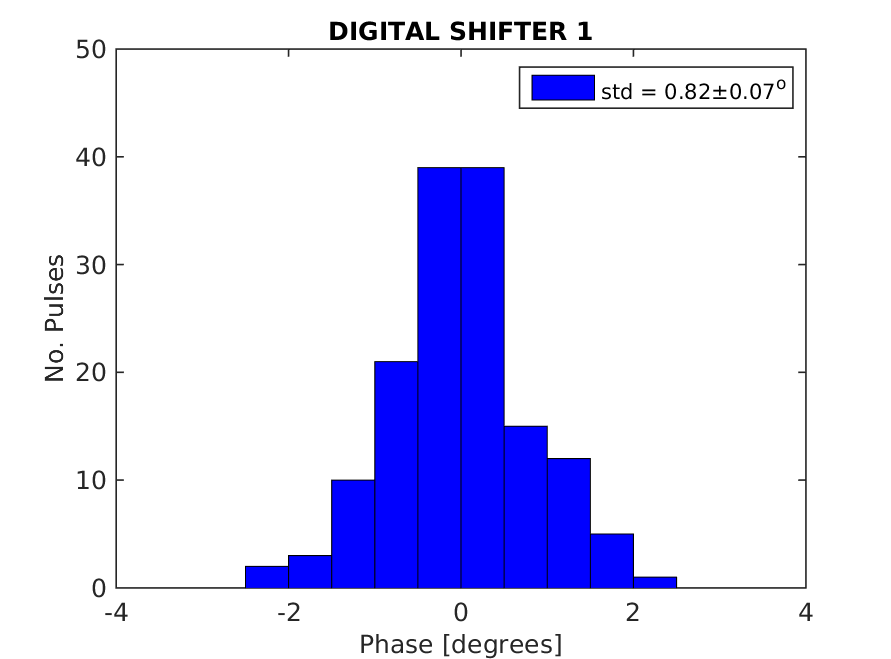
\includegraphics[width=0.45\textwidth]{Figures/PhMon_HistDig1}
  \caption{Dig shifter 1.}
  \label{f:PhMon_HistDig1}
\end{figure}

\begin{figure}
  \centering
  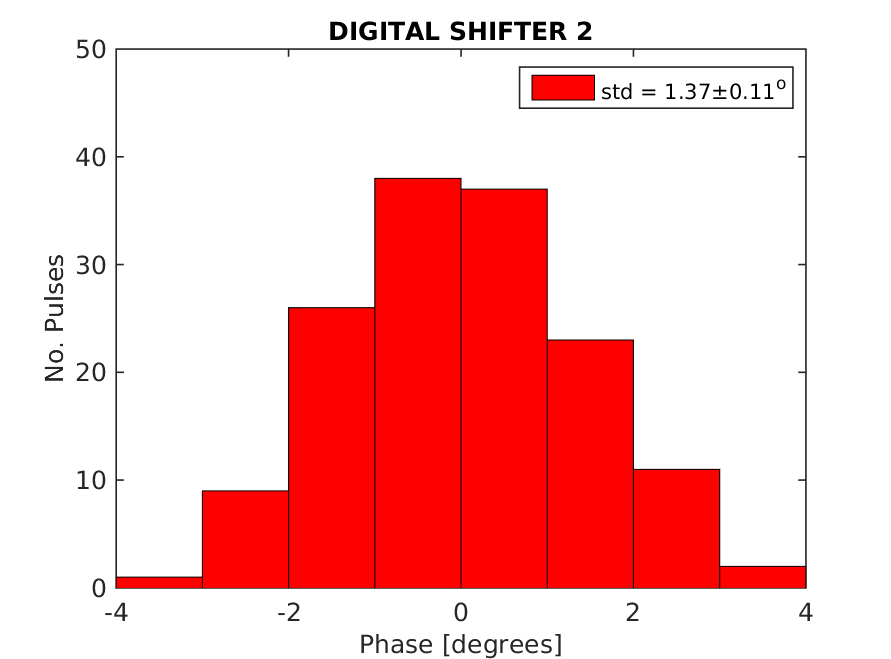
\includegraphics[width=0.45\textwidth]{Figures/PhMon_HistDig2}
  \caption{Dig shifter 2.}
  \label{f:PhMon_HistDig2}
\end{figure}

\begin{figure}
  \centering
  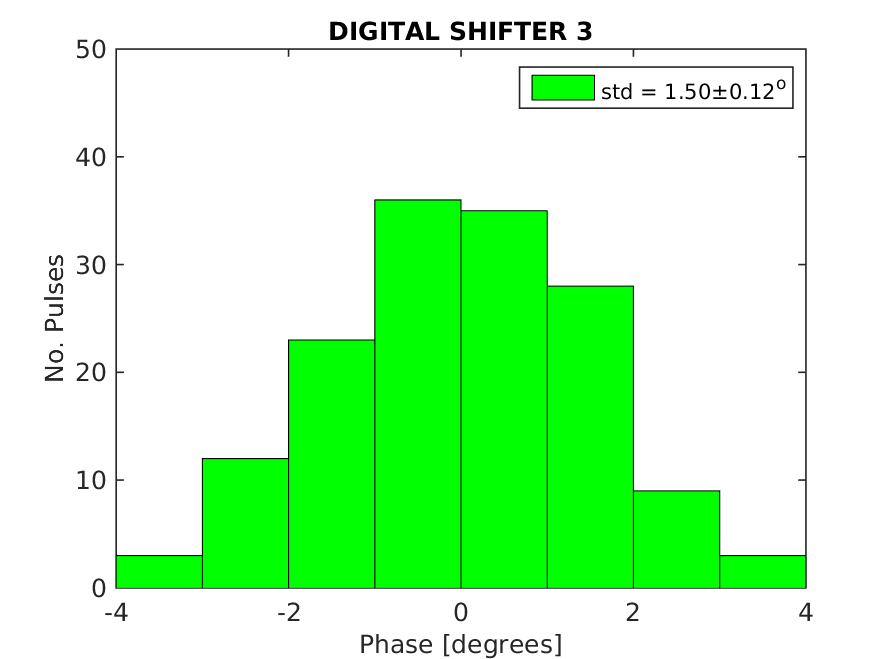
\includegraphics[width=0.45\textwidth]{Figures/PhMon_HistDig3}
  \caption{Dig shifter 3.}
  \label{f:PhMon_HistDig3}
\end{figure}

\subsection{Mechanical Phase Shifters}
\label{ss:mechShiftNoise}

\begin{figure}
  \centering
  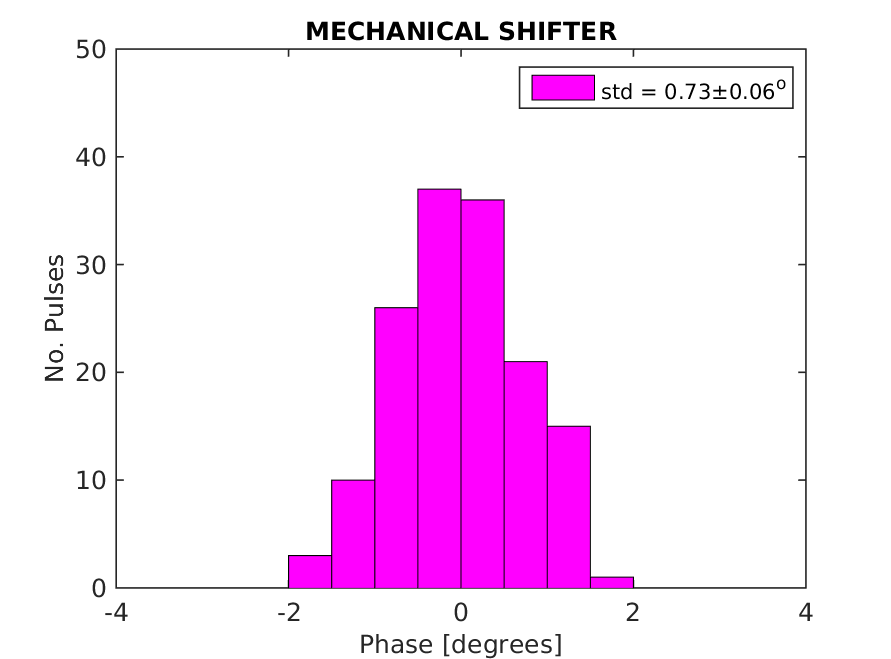
\includegraphics[width=0.45\textwidth]{Figures/PhMon_HistMech}
  \caption{Mech shifter.}
  \label{f:PhMon_HistMech}
\end{figure}

\newsection{s:resolution}{Resolution}

\begin{figure}
  \centering
  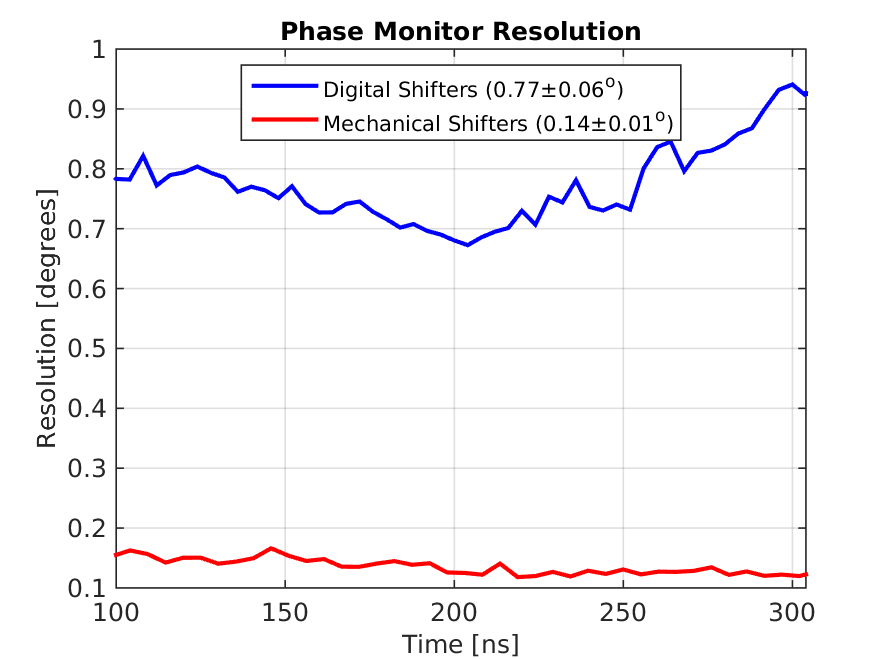
\includegraphics[width=0.45\textwidth]{Figures/PhMon_Resolution}
  \caption{Resolution.}
  \label{f:PhMon_Resolution}
\end{figure}

\newsection{s:monLinearity}{Linearity}

\newsection{s:monBandwidth}{Bandwidth}

\newsection{s:monPosition}{Dependence on Position}








